\chapter{Introduction}\label{ch:introduction}

Placement of the images or paintings on the wall may seem trivial at first.
However, it is not true.
There are different arrangements and constraints to each particular placement.
For example, an art gallery might want to place paintings on the wall, grouping them by their author or style.
One example of such placement can be seen in figure~\ref{fig:london-wall}.
In addition, the room's lighting and the dimensions of the wall and paintings need to be considered.
Together, these requirements pose a complex problem to solve.

\begin{figure}[]
    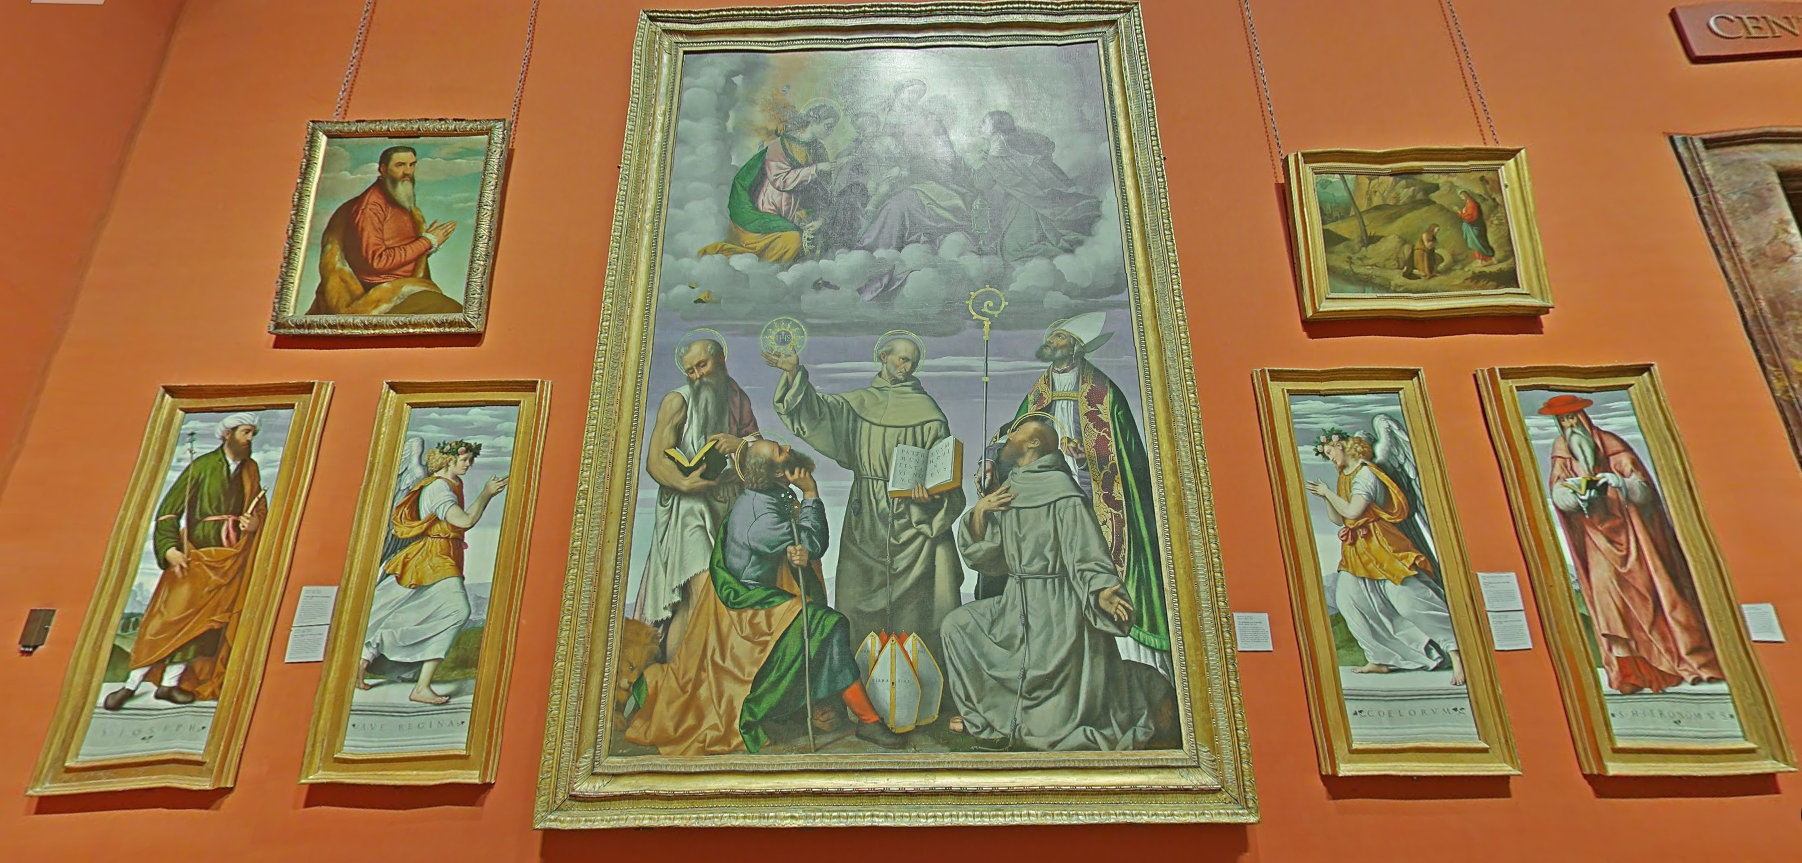
\includegraphics[width=1\textwidth, left]{london_gallery_wall}
    \caption[Painting placement at the London National Gallery]{Painting placement at the London National Gallery. Source:~\cite{ScreenshotWallGoogle}}
    \label{fig:london-wall}
\end{figure}


Furthermore, a solution that places paintings on the wall can be used in many other fields.
For example, the facility layout problem places a set of facilities on a grid
while having the same constraints as the painting placement – grouping related facilities and considering their dimensions~\cite{goncalvesBiasedRandomkeyGenetic2015}.
Another field is retail shelf-space planning, which tries to partition a shelf in a store into rectangles~\cite{yangStudyShelfSpace1999}.
Subsequently, the partitioned shelf is filled with goods that the customers can buy.
Similarly to the lighting conditions for paintings, the placement of goods depends on the
particular placement on the shelf – goods close to the customer's eye level increase their visibility and thus lead to more sales~\cite{hwangGeneticAlgorithmApproach2009}.

The goals of the thesis are:

\begin{enumerate}
    \item Define the painting placement problem, its inputs, constraints, and what a solution to the painting placement problem is.
    \item Create a dataset for the painting placement problem.
    \item Propose and implement a genetic approach for solving the painting placement problem.
    \item Evaluate the performance of the proposed genetic approach.
    \item Discuss the results and suggest further improvements.
\end{enumerate}

The thesis is structured as follows.
Chapter~\ref{ch:literature-review} describes similar problems to the painting placement problem and their solution methods.
They are facility layout problem, shelf-space planning, and sheet metal cutting.
Chapter~\ref{ch:problem-statement-and-formulation} defines the painting placement problem, its inputs, constraints, and what a solution to the painting placement problem is.
The central part of the thesis is in chapter~\ref{ch:coding-and-layout-construction}.
This chapter describes the proposed genetic approach and the construction of the solution to the painting placement problem.
Chapter~\ref{ch:computational-results} evaluates the performance of the proposed genetic approach
and presents the generated dataset.
Chapter~\ref{ch:discussion} discusses the results and suggests further improvements and future work.
Lastly, chapter~\ref{ch:conclusion} concludes the whole thesis.
There is also an appendix~\ref{ch:appendix}, which contains figures and listings outside the thesis's main part.
